\label{MySection 1}
\section{Introduction}

In this section introduce the subject of the project. Provide a broad perspective on the subject area.


\label{MySubSection 1}
\subsection{Creating a sub section}
This is how you add a subsection.
The label command at the beginning of the subsection is used in referencing. (Look at the text)

To reference a section use the ref command. For example this is a reference to section \ref{MySubSection 1} (Look at the text)


\label{MySubSection 2}
\subsection{Creating another sub section}
This is how you add another subsection.


\label{MySubSubSection 1}
\subsection{Creating a sub sub section}
This is how you add a sub subsection. (Look at the text)

The label command at the beginning of the section is used in referencing. (Look at the text)

To reference a section use the ref command. For example this is a reference to the sub section \ref{MySubSubSection 1} (Look at the text)


\label{MySubSection 3}
\subsection{Adding Citations}

For convenience I have created a file called bibliography.bib. In this file are to be found the Bibtex references. If you want to add a reference to the document add it to this file. You may have to regenerate the bibtex references (press F11).

References are included in a document by using the bibliography command. For an example look at the file references.tex.
The style of referencing is set by the command bibliographystyle. For an example see the file main.tex.

To site a reference use the cite command. Here is an example \cite{Rie71}
Here is another example \cite{Ful83}.
The format of the citation is determined by the bibliiography style.


\label{MySubSection 1}
\subsection{Adding figures}

Here is you add figures. Notice the placement of the label and caption commands For simplicity I suggest that you use the Insert Figure Wizard (Under the Wizards menu).

\begin{figure} [hbtp]
\begin{center}
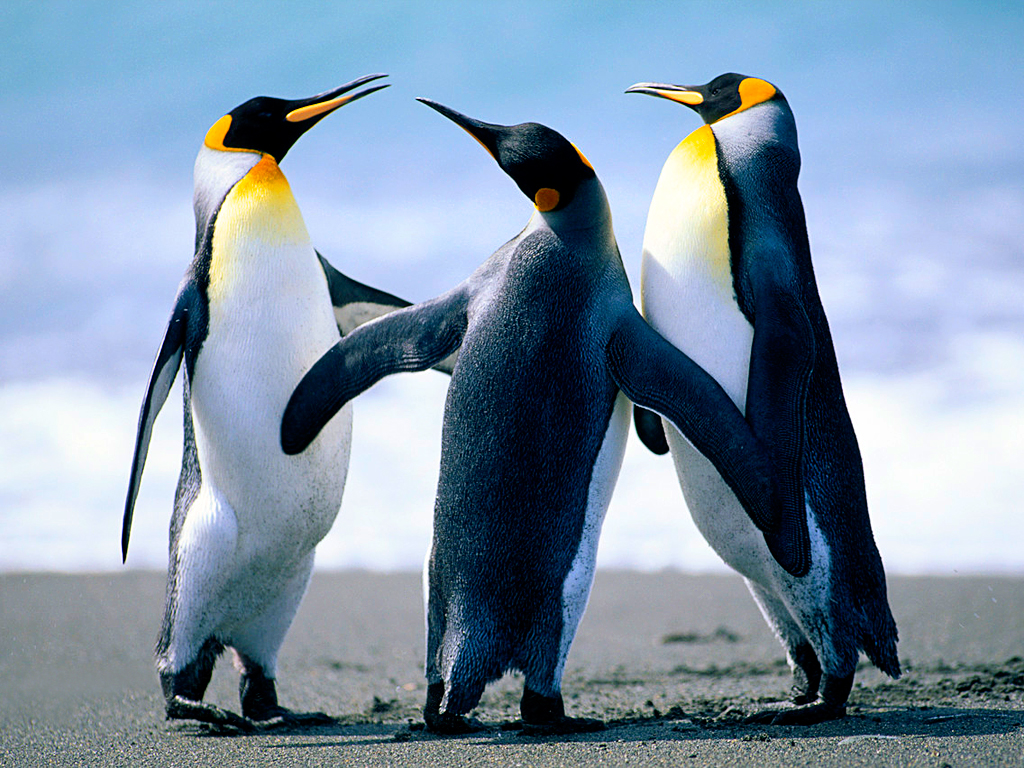
\includegraphics[width=12cm]{./images/Penguins}
\end{center}
\caption{Three student penguins having an important discussion, "What do you mean dude? Adele owns ..."}
\label{figPenguins}
\end{figure}

Here is how you reference the label \ref{figPenguins}


Here is another figure.

\begin{figure}[hbtp]
\centering
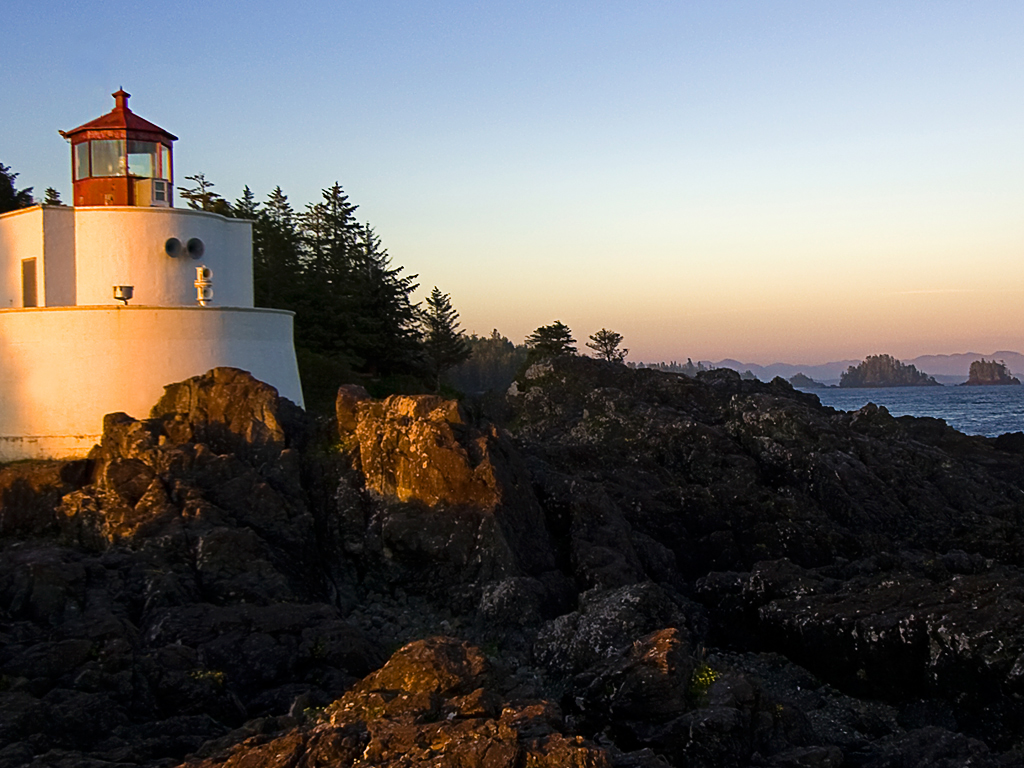
\includegraphics[width=12cm]{./images/Lighthouse}
\caption{Lighthouses ... only look good in pictures and wallpapers. Debate.}
\label{figLighthouse}
\end{figure}

Here is another reference the figure label \ref{figLighthouse}

In the next section we shall look at equations ...
